\chapter{Event Reconstruction}

    \section{Introduction}
        Once a bunch-crossing event has cleared the Level 1 Trigger system, the process of event reconstruction begins.
        An event in ATLAS is, initially, nothing but a collection of electrical signals emitted from the various detectors.
        Event reconstruction is the process wherein detector readings are aggregated together into meaningful patterns,
            which are interpreted as physical objects and processes.
        The key objects of interest in this analysis are \textit{particle tracks} and \textit{jets}.
        As well, the process by which b-quark-originating jets (``b-jets'') are distinguished from other jet types,
            called \textit{flavour tagging}, plays a particularly critical role in this analysis.
        Finally, special attention will be given to the fact that reconstruction occurs not once, but twice;
            first in the High Level Trigger online running environment,
            and again in the offline environment after events have been read out.
        The ways that reconstruction differs between these two environments plays a subtle but important part
            in later stages of this analysis, and so is worth discussing further.


    \section{Tracks}
            
            %Intro about tracks being the first things we see because they're assembled from the inner detector or something.
            %Also I should probably explain what a track is...
        \subsection{Track Definition}
            
            The first point of contact for anything leaving the interaction region of ATLAS is the tracking detectors.
            Consequently, the objects reconstructed from the tracking detectors will be the first point of discussion.
            Prior to encountering the ATLAS calorimeters, particles exiting the IR travel along a relatively unimpeded trajectory.
            Thanks to the inclusion of the Solenoid Magnet field encompassing the Inner Detectors,
                these trajectories reveal crucial information about the particles in an event.
            This is due to the fact that any charged particle, with a momentum component orthogonal to a magnetic field,
                will trace out a \textit{helical} trajectory.
            If the shape of the helix is known, then basic electrodynamics principles can be used to determine the
                momentum and charge of the particle that formed it.
            Specifically, for a particle with four-momentum given as 
            \begin{equation}
            p = \minimatrix{E \\ p_T \\ \theta \\ \phi}
            \end{equation}
            the track's helical shape can reveal all components except for the energy $E$ (this will be handled by the calorimeters).
            To understand how this is achieved, it is worth discussing how a track helix is described mathematically.
            A helix can be described using five parameters structured in a parametric equation.
            There are several conventions for the form these parameters should take,
                but in ATLAS a helix is described by the equations\cite{thesis_giacinto}:
            \begin{equation} \begin{split}
            x(\alpha) &= d_0 \cos(\phi) + \rho \left[ \cos(\alpha) - \cos(\phi) \right] \\
            y(\alpha) &= d_0 \sin(\phi) + \rho \left[ \sin(\alpha) - \sin(\phi) \right] \\
            z(\alpha) &= z_0 - \rho \cot(\theta) (\alpha - \phi)
            \end{split} \end{equation}

            The helix is described relative to the Interaction Region's origin.
            The five parameters governing the shape of this helix, called \textit{perigee paramters}, 
                are described largely in terms of the ``Point of Closest Approach'' (PoCA),
                the point on the helix closest to the PV in the $x,y$ plane.
            \begin{itemize}
                \item $d_0$: $|(x,y)|$-Distance from the origin to the closest point on the helix, in the $x,y$ plane
                \item $z_0$: $z$-Distance between the PoCA and the origin
                \item $\phi$: Angle in the $x,y$ plane of the PoCA
                \item $\theta$: The angle of the helix's trajectory in the $\rho,z$ plane
                \item $\rho$: The radius of curvature of the helix
            \end{itemize}

            \begin{figure}
                \subfloat[Perigee Parameters]{
                    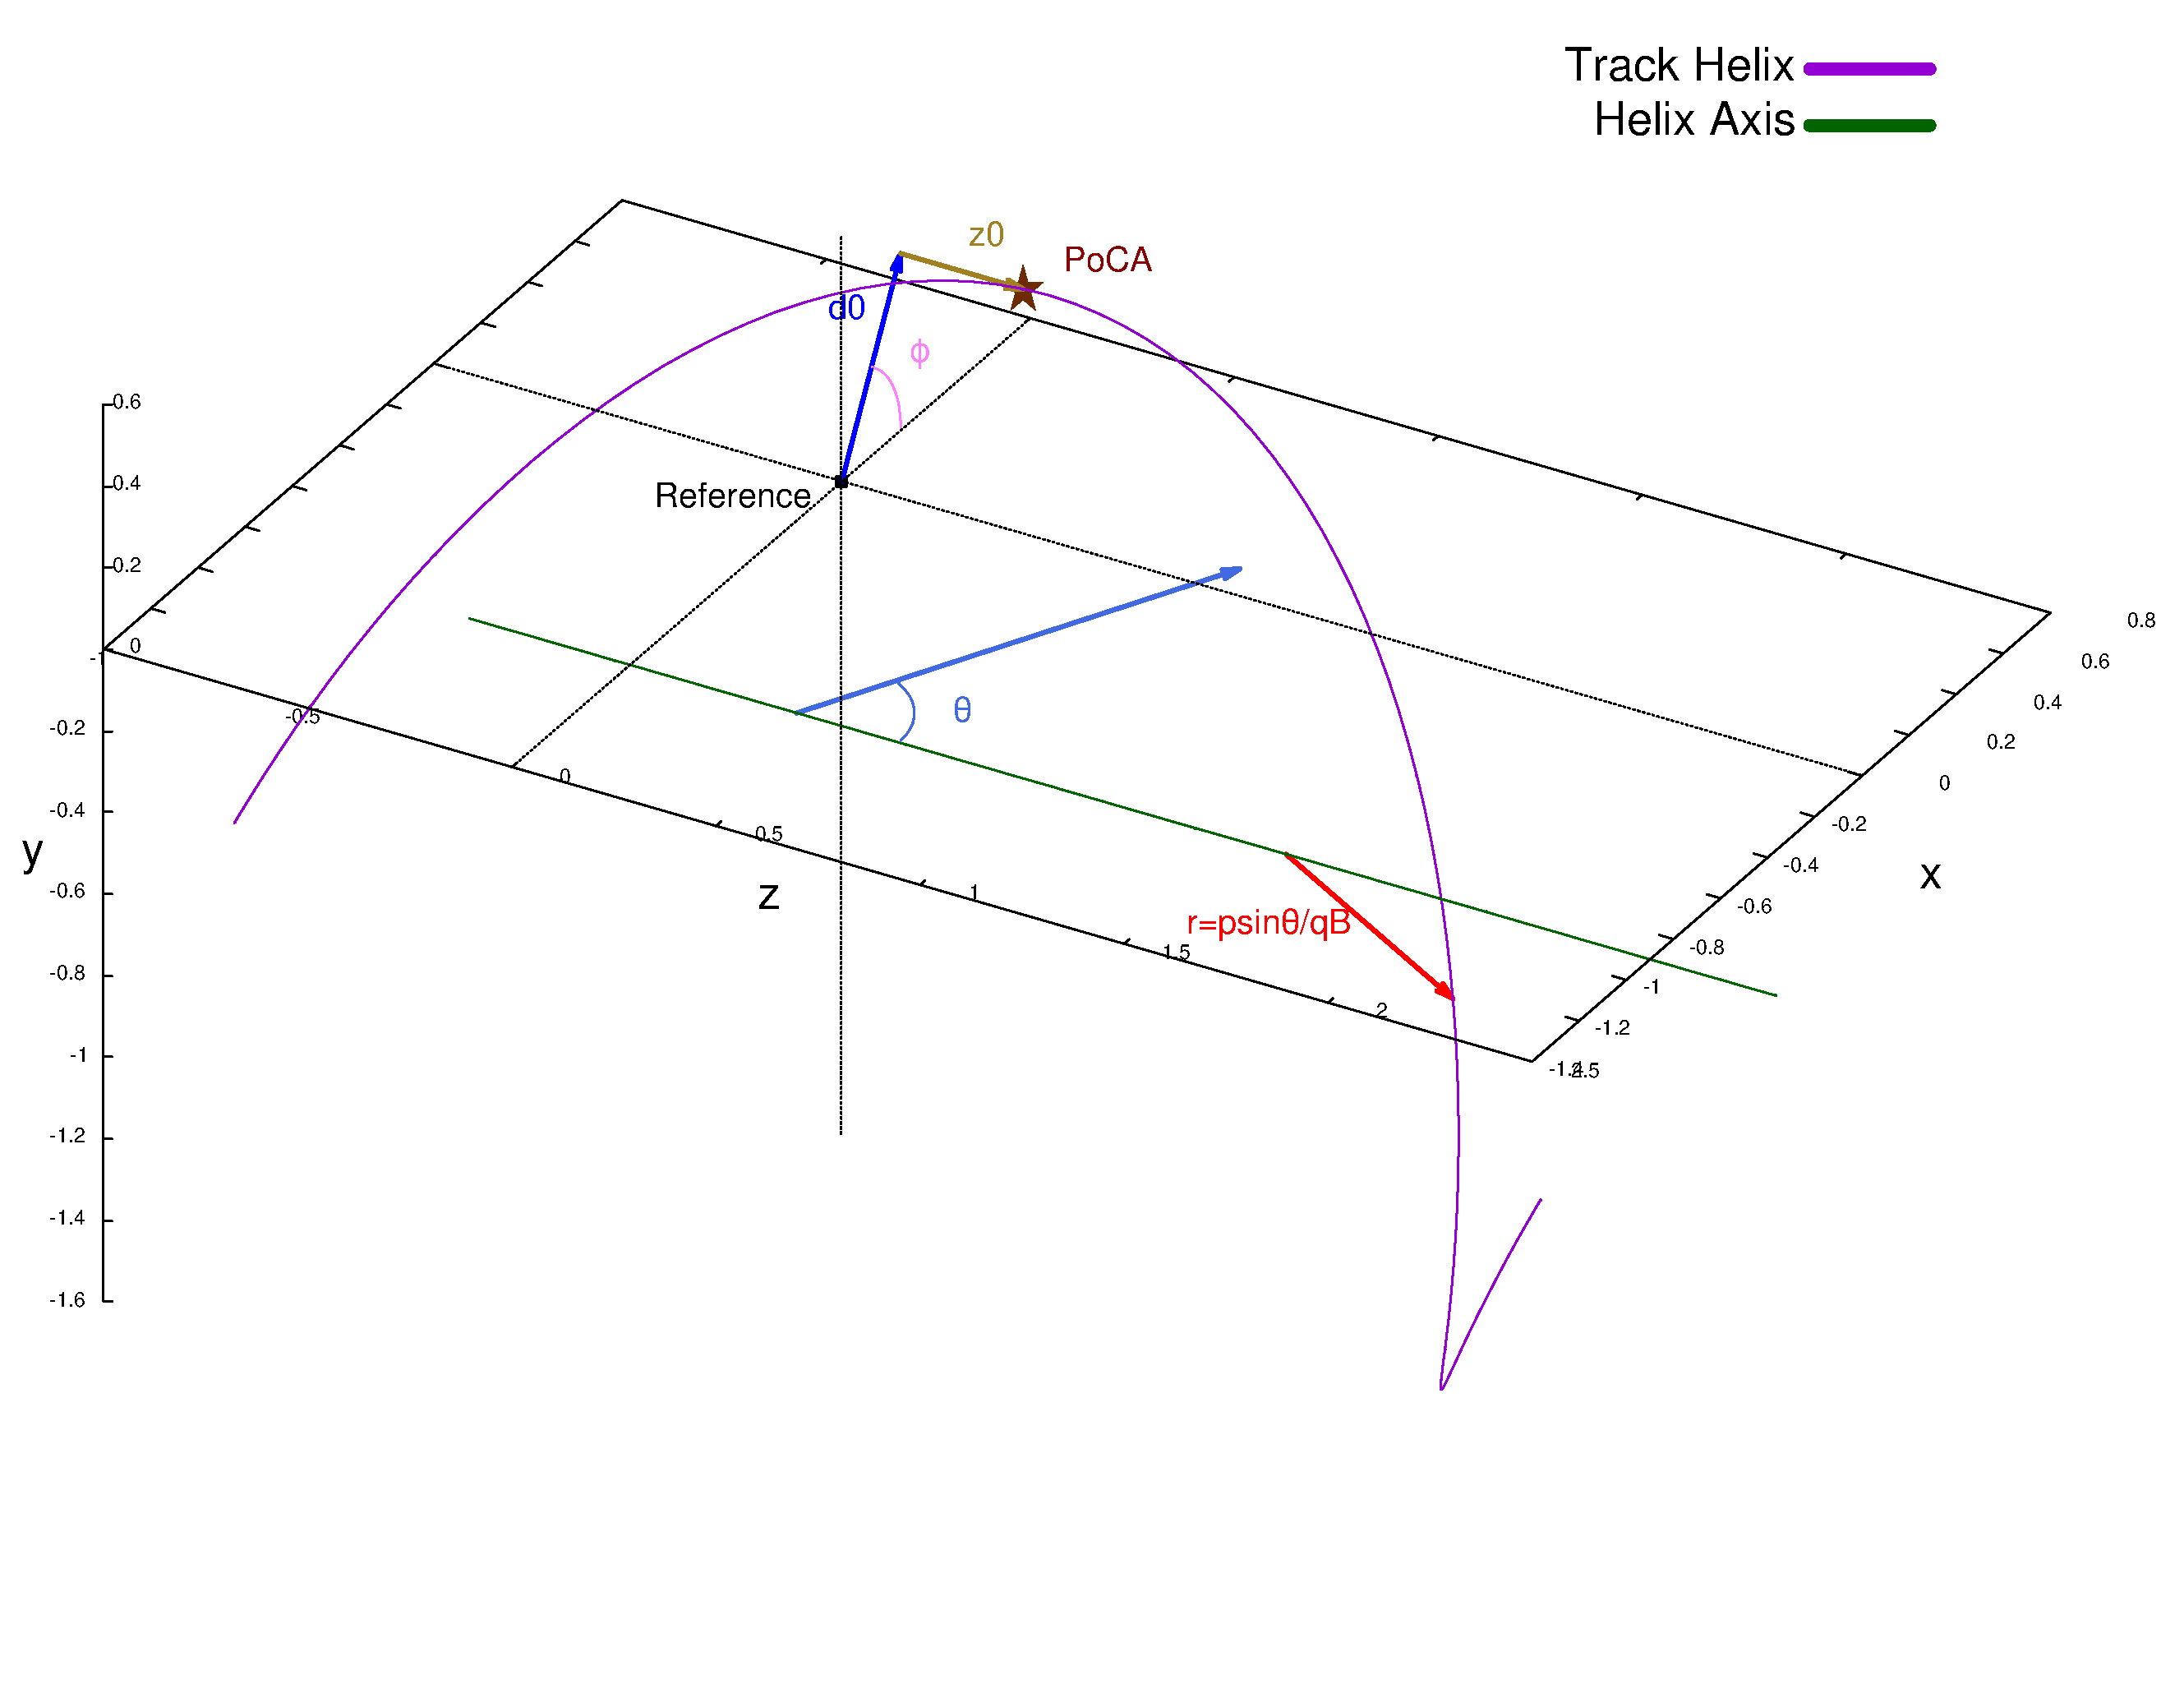
\includegraphics[width=0.5\linewidth,height=\textheight,keepaspectratio]{reconstruction/perigee_base}
                }
                \subfloat[Front View, $(x,y)$-Plane]{
                    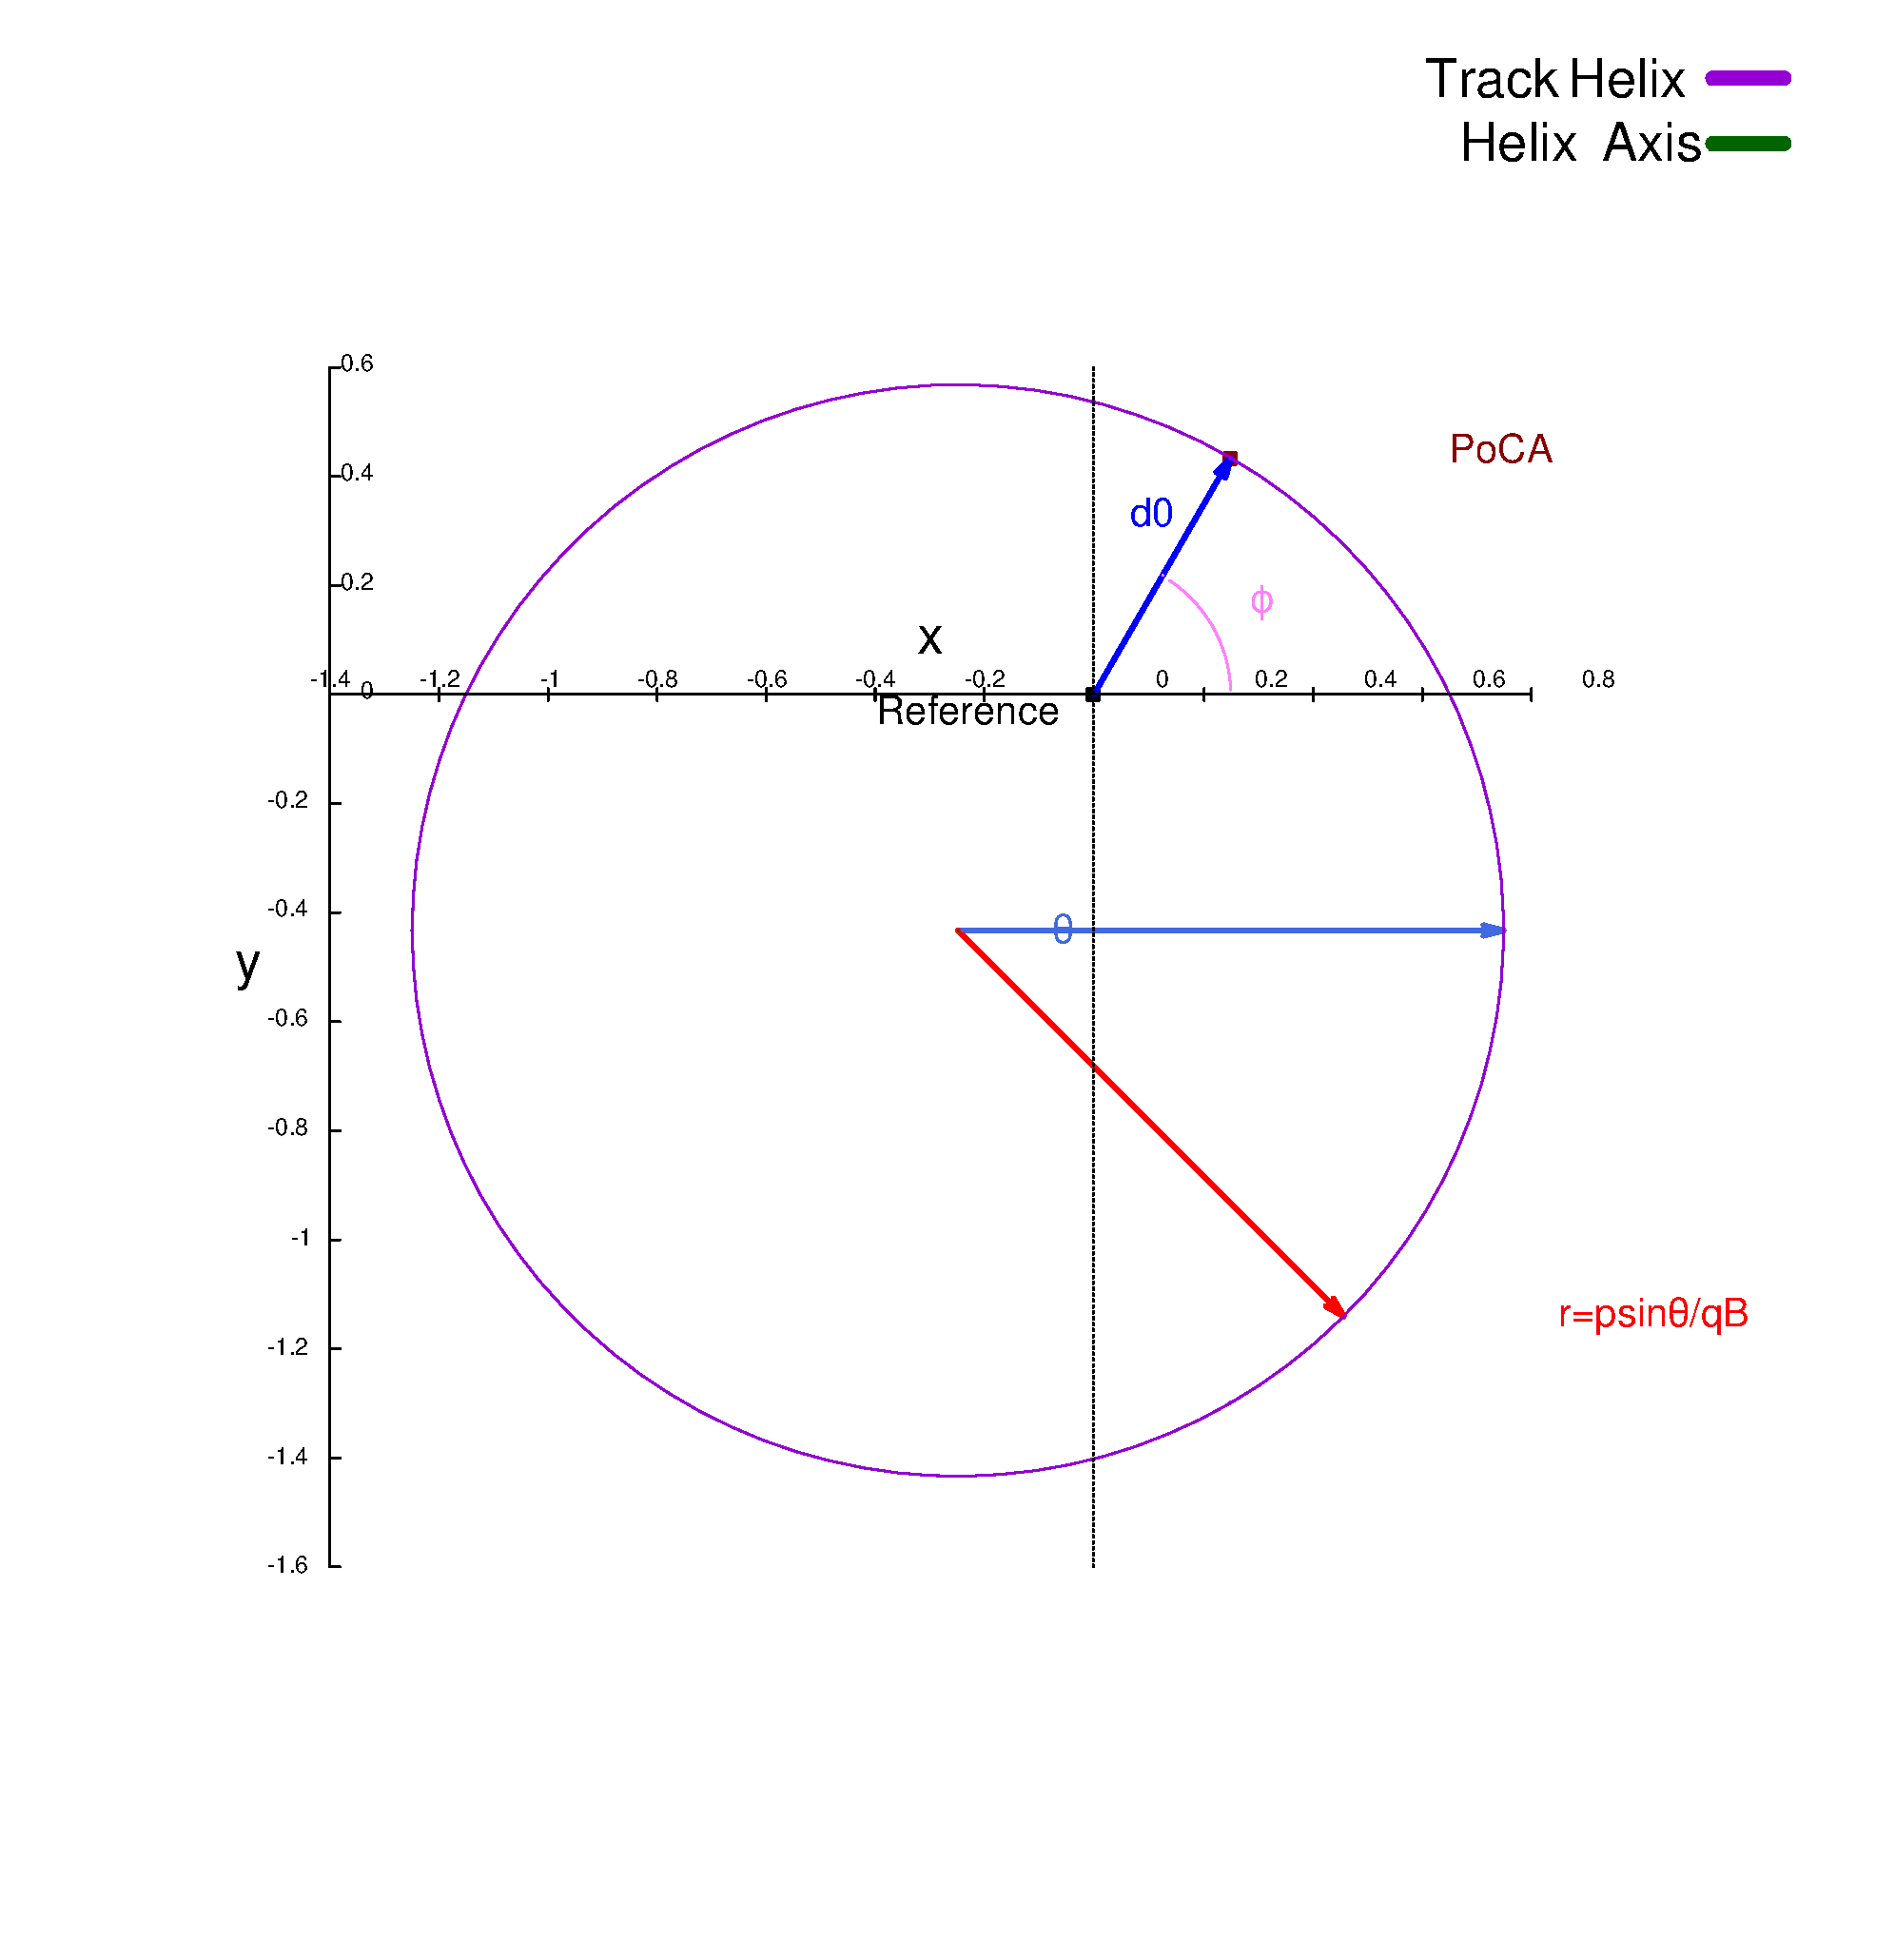
\includegraphics[width=0.5\linewidth,height=\textheight,keepaspectratio]{reconstruction/perigee_front}
                }\\
                \subfloat[Top View, $(x,z)$-Plane]{
                    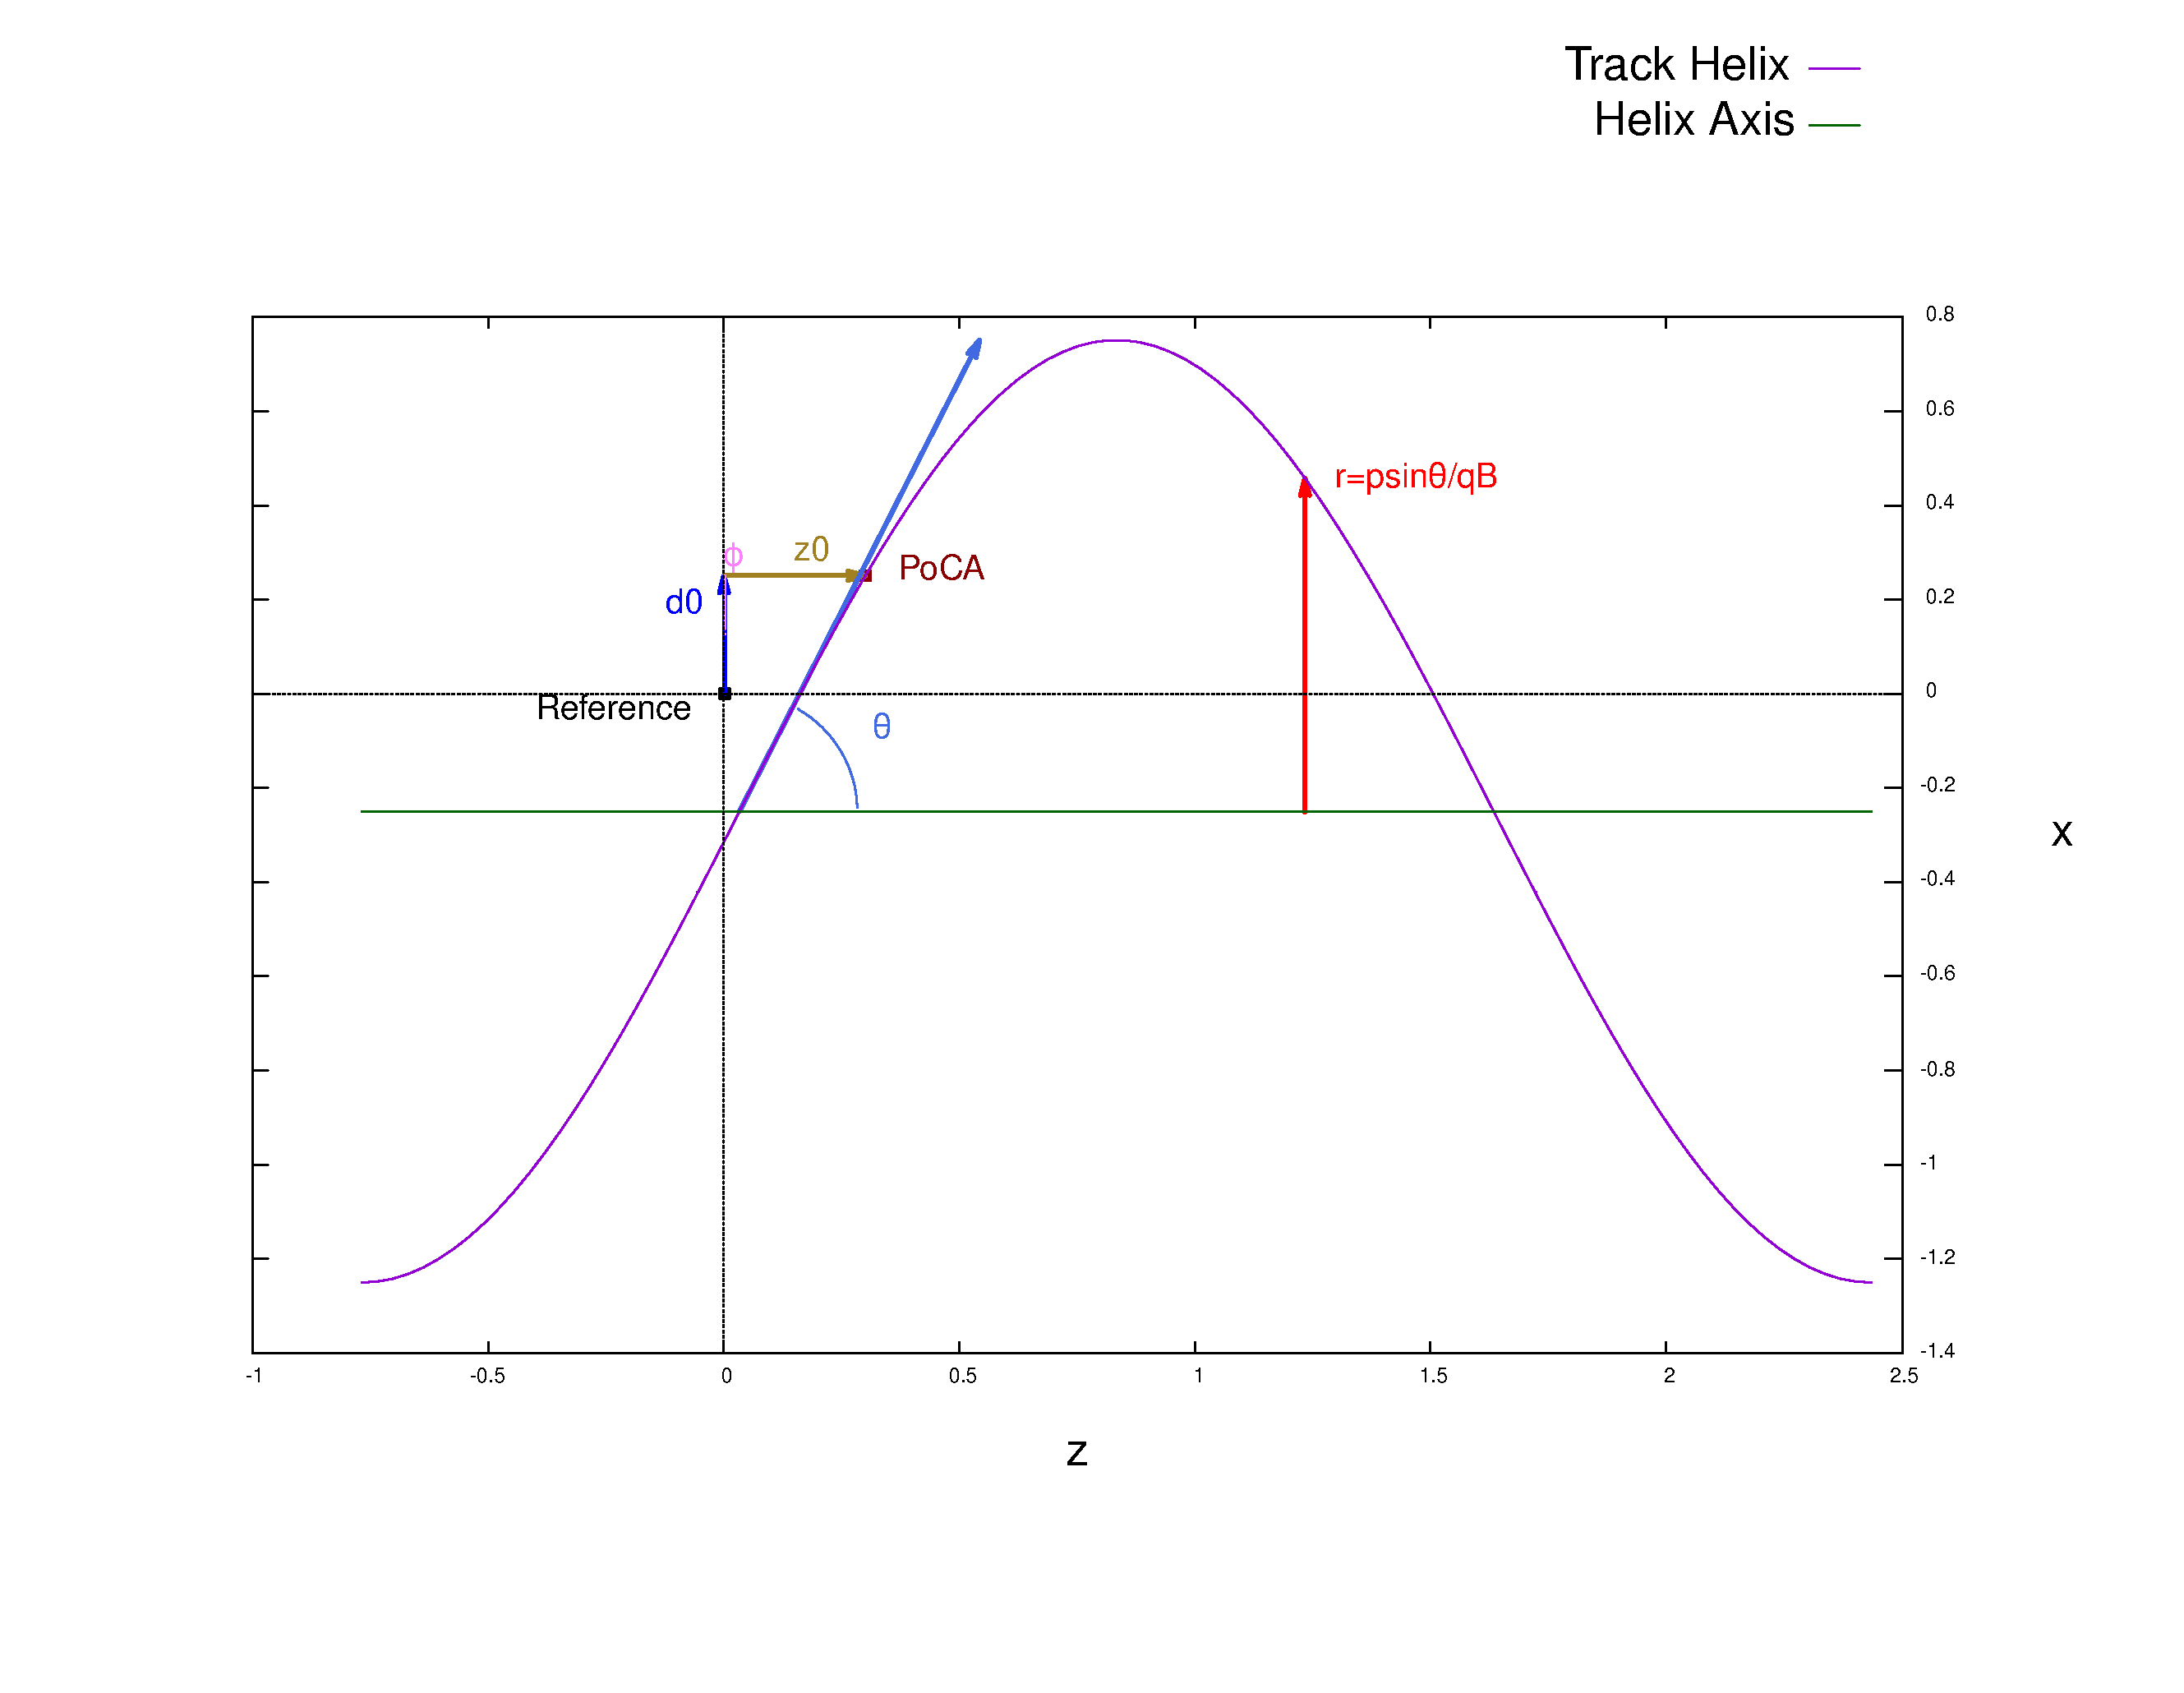
\includegraphics[width=0.5\linewidth,height=\textheight,keepaspectratio]{reconstruction/perigee_top}
                }
                \caption{
                    Perigee parameters are hard! Also I need to replace PV with just Origin, since the PV comes later (oops).
                }
                \label{fig:perigee_params}
            \end{figure}
            

            Both $d_0$ and $z_0$ will be used in later sections for the purpose of flavour tagging.
            Returning to the four-momentum, $\phi$ and $\theta$ are themselves components of the particle's 4-vector.
            The final parameter, $\rho$ can then be related to the particle's tranverse momentum and electric charge as
            \begin{equation}
            r = \frac{p_T}{qB} = \frac{\vec{p} \sin(\theta)}{qB}
            \end{equation}
            where $B$ is the magnetic field of the Inner Detector Solenoid Magnet.
            \cite{thesis_track_sim_and_reco}

        \subsection{Track Reconstruction}

            As particles pass through the inner detector subsystems, they trace out a path of ionized detector elements.
            The trajectory can be reconstructed by playing connect the dots.

            %Clusterization
            The first step to producing a track is the process of clusterization.
            Ionizing particles often deposit energy across several adjacent pixels on a given layer.
            A \textit{connected component analysis} algorithm is used to group pixels together.
            Based on the pattern of energy distribution in these groups,
                a \textit{space-point} is created indicating the estimated position at which a particle crossed the detector.
            Several space-points can be assigned to the same pixel cluster,
                if the energy readout pattern suggests multiple particles traversed the same location.

            %Combinatorial track finding
            Initial guesses at tracks, called track seeds, are formed by assembling all realistic combinations of three space-points.
            The track seeds are assigned helix parameters by assuming they travel through a uniform magnetic field,
                allowing immediate estimates of the tracks' momentum.
            These seeds are expanded into \textit{track candidates},
                by including more space-points across additional detectors in the ID using a \textit{Kalman filter}.

            %Ambiguity solving; NN clustering; Track fit
            A number of criteria are then used to reject poor-quality tracks, as well as to assign scores to all remaining track candidates.
            The scores are then used to resolve ambiguities where multiple tracks are assigned to the same space-points,
                with preference given to higher-scoring candidates.
            Neural networks are used to assist in some ambiguity solving situations,
                as well as to help identify clusters with multiple valid tracks.
            Once ambiguities have been resolved and all malformed track candidates removed,
                the remaining tracks are refit using all available information at high-resolution\cite{atlas_track_reco_performance}.

    \section{Jets}
        Moving outwards from the inner tracker into the calorimeters, focus shifts from tracks to the reconstructed objects known as \textit{jets}.
        Jets are an attempt to encapsulate the process of scattering within high-Z materials.
        A high energy particle encoutering the heavy-metal plates in the calorimeters will be deflected,
            while releasing other particles which travel in different directions.
        All these new particles will produce similar reactions, until the various particles posses too little energy to produce any more scattering.
        The overall effect appears as a cone-shaped shower of particles,
            whose ``tip'' is located at the original particle's point of entry into the calorimeters.
        This cone has an associated vector corresponding to the direction the cone opens out at.
        Due to conservation of momentum, the momentum vector of the original particle will be roughly equal to the jet vector,
            since the total momentum of the various scattered particles must sum back to the momentum of the initial particle.

        Though jets are meant to represent a physical phenomenon,
            it should be emphasized that jets themselves \textit{are not physical objects}.
        Rather, jets are an algorithm.
        Specifically, jets are an algorithm used to cluster different cells in a calorimeter together,
            based on the energy deposited in each cell.
        The general goal is to have each complete ``topological cluster'' (topo-cluster) correspond to one particle.
        In practice however, particles frequently overlap in their energy deposition,
            making it challenging to distinguish where one cluster should begin and another should end.
        Historically, a number of different jet algorithms have been used to describe particle showers.
        In ATLAS, the jet algorithm currently in use is the \textit{\antikt} clustering algorithm\cite{anti_kt},
            whose adoption has been motivated by its robust ability to isolate jet boundaries both from each other
            and from the surrounding stochastic noise of the detector.
        [NOTE: Hey Steve, do I need to describe how antikt works?
        It's not that complicated, but it's kinda weird and unintuitive and I'm not sure if its description would add much]

        Once topo-clusters have been formed, their energy and momentum must be calibrated.
        As discussed in Section \ref{sec:calorimeter}, the ATLAS calorimeters are sampling calorimeters.
        This means that the bulk of energy deposited is lost in inactive material, and not read out.
        Additional energy losses are incurred from inefficiencies in the clustering algorithm and from the \textit{non-compensating} nature of ATLAS calorimeters.
        That is, they do not have an intrinsic method to acount for the fact that electromagnetic radiation deposits a higher fraction of its energy into the detectors than hadronic radiation\cite{cell_clustering}.

        After correcting for energy, the next step is to correct for momentum.
        This is achieved by making a key assumption in reconstruction, related to the \textit{Primary Vertex}.
        When bunches collide in the IR of ATLAS, most of the collisions of a given bunch are fairly minor.
        Events which clear the L1 trigger however, typically do so because of the presence of a hard-scatter interaction.
        Identifying the location along the beamline at which this hard-scatter interaction occured is achieved via ``vertex-finding.''
        Points along $z$ from which particles originate are reffered to as ``vertices''.
        They are identified in reconstruction by tracing the aformentioned tracks backwards
            and identifying points at which they intersect the $z$-axis.
        Most of the vertices are of little interest, and are known as Pile-up vertices.
        The vertex assumed to be associated with the hard-scatter interaction, called the Primary Vertex (PV),
            is identified as a vertex which is associated with two tracks,
            and whose tracks posses the largest sum of squared momentum\cite{jet_energy_scale13TeV}.
        Reconstructed jets are assumed to originate from the hard-scatter interaction point.
        Thus, the momentum vectors associated with the jets and their topo-clusters are adjusted to point back from the PV.

        As a final step in the jet reconstruction process for this analyis comes the track-matching algorithm.
        To improve the performance of reconstructing hadronic jets,
            the various jet vectors are each matched to a corresponding track that the jet likely started from.
        This algorithm, called \textit{Particle Flow} treats the jets as extensions of the reconstructed particles,
            matching jets to tracks based on both location and energy projections.
        The resulting jet-track combination objects are known as \textit{PFlow Jets},
            which are then used for the rest of the reconstruction process\cite{pflow}.

        %Jets created using only calorimeter-based topological-clusters (at the electromagnetic scale [what does this mean??]) %TODO?
            %are reffered to as \textit{EMtopo Jets}. %I still don't really get this, and I'm not sure they're even really used, so imma skip it

    \section{Flavour Tagging}
        
        There are many kinds of particles and processes that can produce jets.
        One particular kind of jet which is integral to this analysis is that of b-quark-initiated jets,
            more simply known as b-jets.
        B-jets are important because, of all the particles the Higgs can decay to,
            its branching ratio to a $\bbar$ pair is highest.
        Distinguishing b-jets from other jet types,
            achieved through the process of \textit{flavour tagging},
            is therefore of paramount importance in this analysis.
        Flavour Tagging in ATLAS is performed in two stages;
            first with a set of simple low-level taggers,
            and then with a set of more sophisticated taggers which use the low-level tagger information as inputs.

        \subsection{Impact Paramter Taggers}

            The low-level b-tagging algorithms come mainly in the two forms of impact parameter taggers and vertex algorithms.
            IP2D and IP3D are the two and three-dimensional impact parameter-based taggers.
            They take advantage of the fact that b-quarks are significantly longer lived than light and charm quarks,
                and thus their associated tracks typically have larger impact parameter values.
            They take every track associated with a PFlow Jet,
                and then use a slightly modified version of the perigee parameters discussed above in order to tag it.
            Namely, the $d_0$ and $z_0$ parameters are given a positive or negative sign to help better emphasize key characteristics of b-jets.
            [explain the sign convention.]
            Physically, this sign convention is to distinguish tracks which are likely to have actually been part of the jet (with a positive sign)
                from those likely originating from pile-up vertices (negative sign).
            Values are associated with \textit{each} track in a jet based on probability density functions (PDF) of the different jet types.
            IP2D and IP3D are then constructed as likelihood ratios of the product of all track-values $t_i$for a jet.
            For example, the likelihood ratio of a jet being a b-jet versus a light-jet would be based on
                the PDF of the impact parameter for b-jets ($\textrm{PDF}_b$) to that for light-jets ($\textrm{PDF}_l$)

            \begin{equation}
                R(t_1, t_2, ... t_N) \equiv \frac{\prod_{i=1}{N} \textrm{PDF}_b(t_i)}{\prod_{i=1}{N} \textrm{PDF}_l(t_i)}
            \end{equation}

            These distributions are then used as a discriminant to distinguish b-jets from charm and light-jets
                (see Figure TODO)\cite{thesis_giacinto}.

        \subsection{Secondary Vertexing Algorithms}

            Vertex Algos - SV1 (Secondary Vertex 1) and JetFitter

        \subsection{High Level Taggers}

            MV2, a Boosted Decision Tree (BDT);
            DL1, a Deep Learning Neural Network (DL1r is what we specifically use)
            \cite{bjet_id_and_performance}
            \cite{btagging_optimisation}

    \section{Online VS Offline Reconstruction}
        I should explain how online and offline reco differs;
            it seems to just come down to the fact that the HLT doesn't neccesarily use the most high resolution calorimeter information,
            and often generates tracks using a faster, less acurate algorithm.

        Reconstruction is performed for an event twice.
        It is first done rapidly, using coarse measurments and calculations,
            for the purpose of allowing the aforementioned HLT to trigger events for readout.
        These events which pass the trigger are passed off to a massive global computer cluster reffered to as the GRID.
        No longer bound by the stringent time contrainsts of the ``online'' running environment,
            the GRID is able to devote vast amounts of time and computing power to a second, 
            more comprehensive, reconstruction of each event.
        For both the ``online'' (HLT) and ``offline'' (GRID) environments, event reconstruction is carried out by the same suite of software,
            called \textit{Athena}.

        %TODO: Do I have ROC curves comparing MV2c10 scores b/t on and offline?
            
        I should also describe the mv2 reweighting procedure here
            (We don't use mv2 for the late-stage b-tag requirement on the higgs decay candidates,
            but we DO use it in the triggers):
            Step1.1 - Run HLT reco on MC files;
            Step1.2 - Return low level taggers on MC HLT reco;
            Step2   - Rerun HLT reco on MC, now with retuned low level tagging info;
            Step3.1 - Perform BDT training for MV2 on HLT MC reco w/ low level tags;
            Step3.2 - Convert training output to useable histograms;
            Step4   - Rerun HLT reco on MC once more, to get full retuned tagging ouput. Use output performance to determine working points;

